\saltoPag{}
\section{UNIDAD 4}
    \begin{center}
        \begin{tabular}{| m{2.25cm} | m{2.25cm} | m{2.25cm} |}
            \hline
            \multicolumn{3}{| c |}{\textcolor{red}{\textbf{ESTADOS DE AGREGACIÓN}}} \\
            \hline
            \multirow{1}{2.25cm}{\centering\textbf{Sólidos}} &
            \multirow{1}{2.25cm}{\centering\textbf{Líquidos}} &
            \multirow{1}{2.25cm}{\centering\textbf{Gases}} \\
            \hline
            Forma definida & Volumen definido & Forma y volumen del recipiente que lo contiene. \\
            \hline
            Volumen definido & Forma del recipiente que lo contiene & Muy compresible \\
            \hline
            No comprensibles & No comprensibles & Movimiento muy libre \\
            \hline
            Partículas ordenadas con movimiento de vibración & Las partículas se deslizan entre sí libremente & \\
            \hline
        \end{tabular}
    \end{center}
    \begin{center} 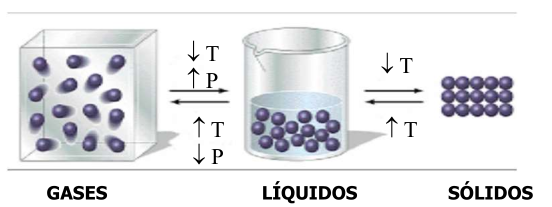
\includegraphics[width=7cm]{./imagenes/estadosDeAgregacionMoleculas.png} \end{center}
    \subsection{Líquidos}
        \subsubsection{Viscosidad}
            \sangria{} Medida de la resistencia de un líquido para fluir.
            \begin{center} 
                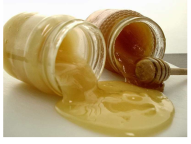
\includegraphics[width=4cm]{./imagenes/miel.png} \\[15pt]
                \textit{El aumento de la temperatura implica menor viscosidad.}
            \end{center}
            \begin{center} 
                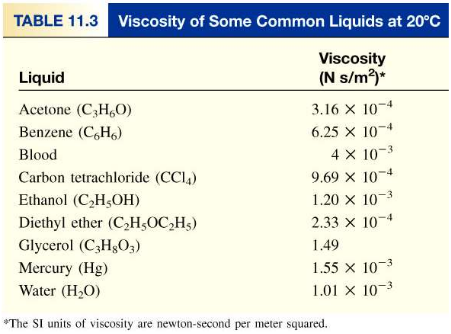
\includegraphics[width=6cm]{./imagenes/tablaViscosidad.png} \\[15pt]
                \textit{Las fuerzas inter-moleculares fuertes implican una alta viscosidad.}
            \end{center}

        \subsubsection{Tensión superficial}
            \sangria{} Cantidad de energía requerida para dilatar o aumentar la superficie de un líquido por unidad de área.
            \begin{center} 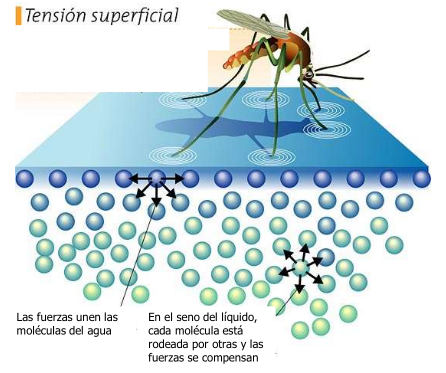
\includegraphics[width=6cm]{./imagenes/mosquitoTensionSuperficial.png} \end{center}
            \begin{center} \textcolor{red}{\underline{Capilaridad:} ejemplo de tensión superficial} \end{center}
            \sangria{} Es el resultado de dos fuerzas:
            \begin{itemize}
                \item \textbf{Cohesión:} atracción inter-molecular entre moléculas similares.
                \item \textbf{Adhesión:} atracción inter-molecular entre moléculas diferentes.
            \end{itemize}
            \begin{center} 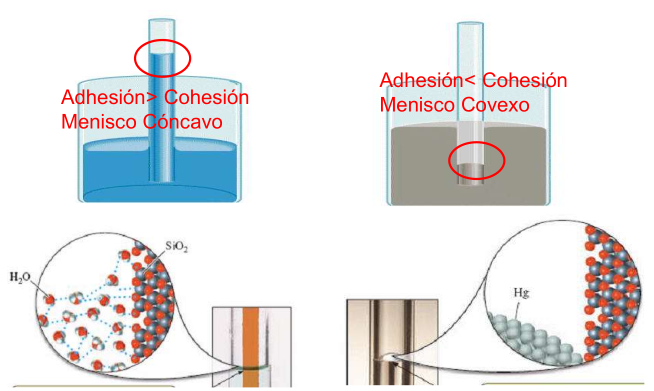
\includegraphics[width=6cm]{./imagenes/fuerzasCapilaridad.png} \end{center}
            \begin{center} 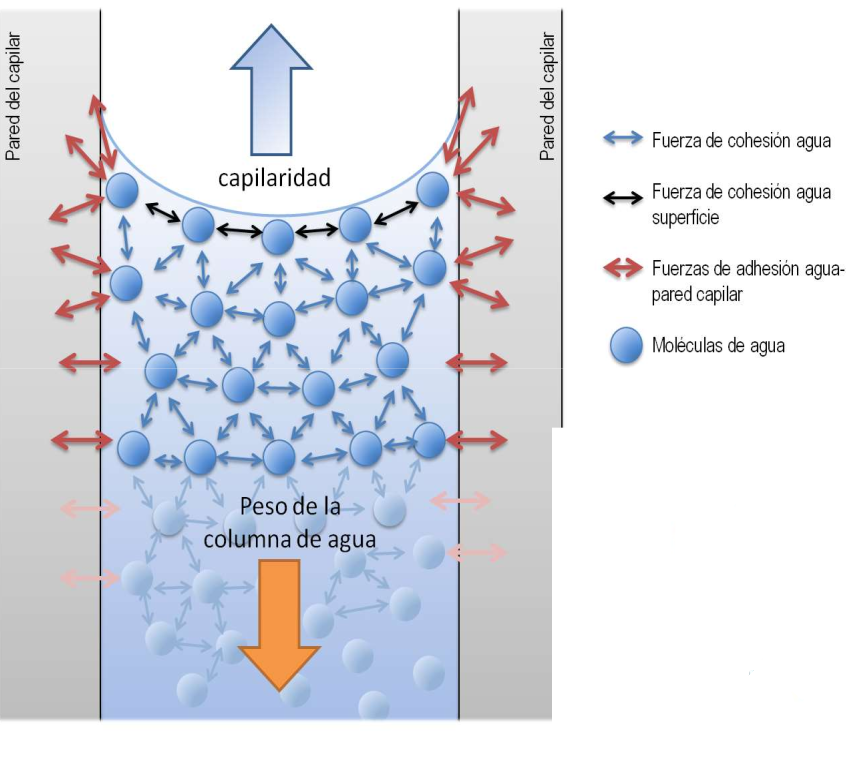
\includegraphics[width=8cm]{./imagenes/detallesCapilaridad1.png} \end{center}
            \begin{center} 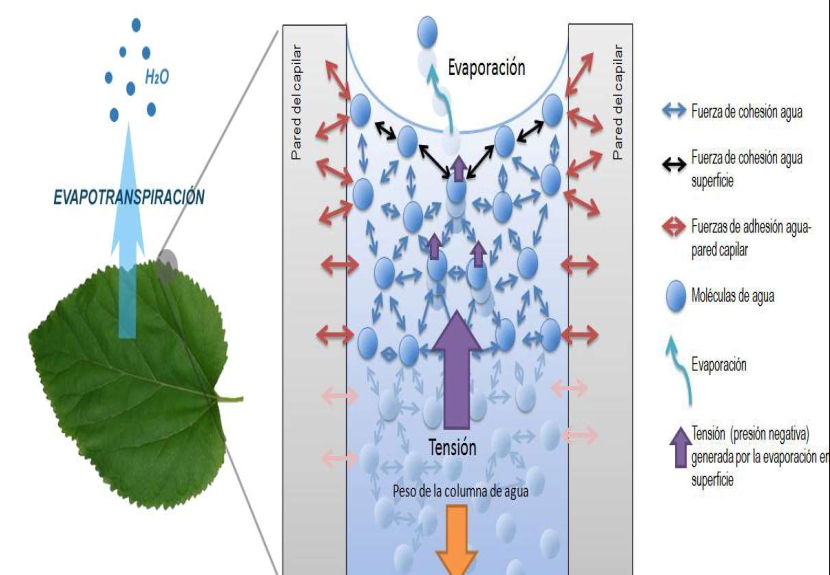
\includegraphics[width=8cm]{./imagenes/detallesCapilaridad2.png} \end{center}
        \saltoPag{}
        \subsubsection{Evaporación y presión de vapor}
            \sangria{} \underline{Conceptos:}
            \begin{itemize}
                \item \textbf{Presión de vapor:} presión ejercida por el vapor de un líquido sobre la superficie del mismo cuando el líquido y el vapor se encuentran en equilibrio dinámico a una temperatura determinada.
            \end{itemize}
            \begin{center} 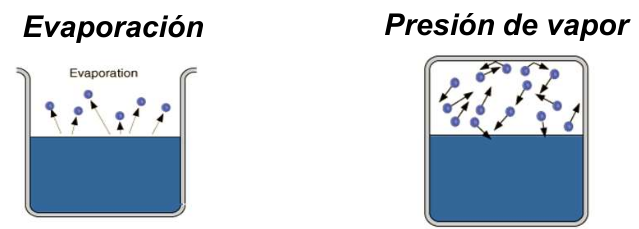
\includegraphics[width=5cm]{./imagenes/evaporacionYPresionDeVapor.png} \end{center}
            \begin{center}
                \begin{tabular}{ | m{1.8cm} | m{1cm} | m{1cm} | m{1cm} | m{1.3cm} |}
                    \hline
                    \multicolumn{5}{| c |}{\textcolor{red}{\textbf{Presión de vapor (Torr)}}} \\
                    \hline
                    \textbf{Compuesto} & \centering $\ang{0}C$ & \centering $\ang{20}C$ & \centering $\ang{30}C$ & \scriptsize \textbf{Punto de ebullición normal ($1atm$)} \\
                    \hline
                    Dietileter & 185 & 442 & 647 & $\ang{36}C$ \\
                    \hline
                    Etanol & 12 & 44 & 74 & $\ang{78}C$ \\
                    \hline
                    Agua & 5 & 18 & 32 & $\ang{100}C$ \\
                    \hline
                \end{tabular}
            \end{center}
            \begin{itemize}
                \item \textbf{Punto de ebullición:} es la temperatura en la cual la presión de vapor (en equilibrio) de un líquido es igual a la presión externa.
                \item \textbf{Punto de ebullición normal:} es la temperatura en la cual un líquido hierve cuando la presión externa es de $1atm$.
            \end{itemize}
            \begin{center} 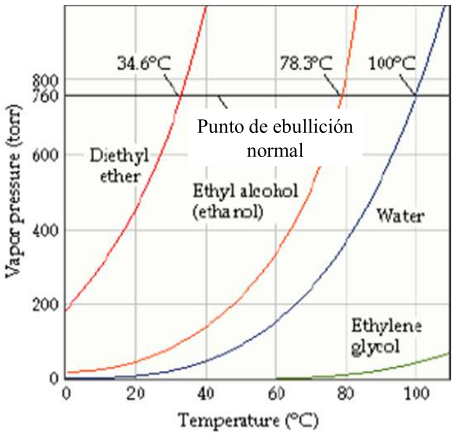
\includegraphics[width=7cm]{./imagenes/puntoDeEbullicion.png} \end{center}
            \begin{itemize}
                \item \textbf{Temperatura crítica ($T_C$):} temperatura por arriba de la cual el gas no puede licuarse, no importa cuán grande sea la presión aplicada.
                \item \textbf{Presión crítica ($P_C$):} es la presión mínima que debe aplicarse para ocasionar licuefacción a la temperatura crítica.
            \end{itemize}
            \begin{center} 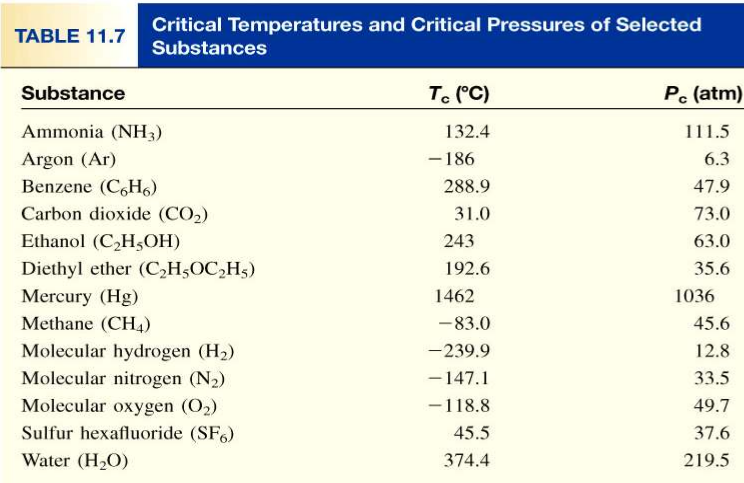
\includegraphics[width=8cm]{./imagenes/presionYTemperaturaCritica.png} \end{center}
            \begin{itemize}
                \item \textbf{Diagrama de fases:} resume las condiciones en las cuales una sustancia existe como sólido, líquido o gas.
            \end{itemize}
            \begin{center} 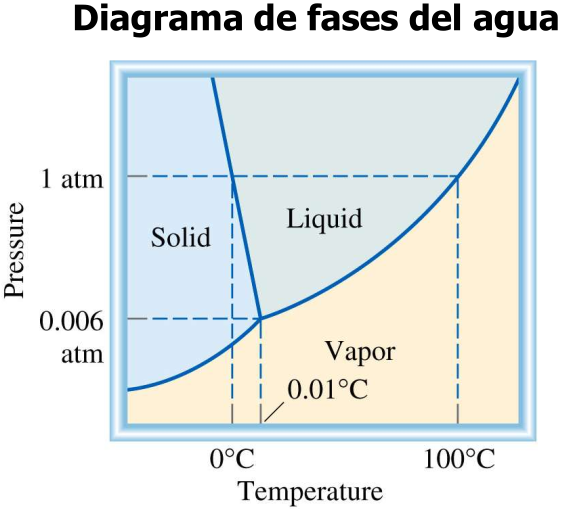
\includegraphics[width=6cm]{./imagenes/diagramaDeFasesDelAgua.png} \end{center}
            \begin{center} 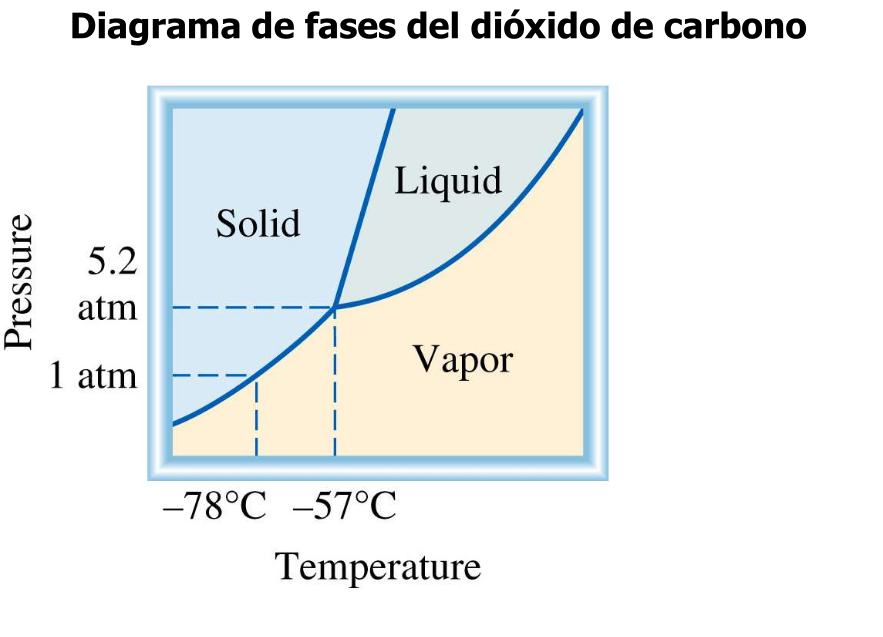
\includegraphics[width=6cm]{./imagenes/diagramaDeFasesDelCO2.png} \end{center}
    \subsection{Gases}
        \sangria{} Los siguientes elementos pueden existir como gases a una temperatura de $\ang{25}C$ y a $1atm$ de presión.
        \begin{center} 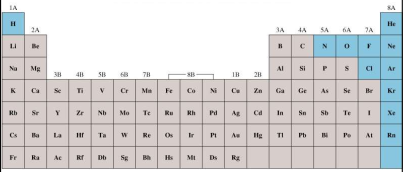
\includegraphics[width=7cm]{./imagenes/elementosGasACondNormales.png} \end{center}
        \saltoPag{}
        \begin{center} 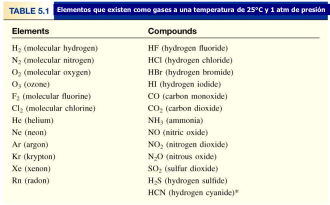
\includegraphics[width=7cm]{./imagenes/elementosGasACondNormales1.png} \end{center}
        \subsubsection{Características físicas de los gases}
        \begin{itemize}
            \item Son capaces de adquirir cualquier forma.
            \item Compresibles.
            \item Pueden mezclarse con todo tipo de elementos con mucha facilidad.
            \item Tienen una densidad mucho menor que los sólidos y los líquidos.
        \end{itemize}
        \subsubsection{Presión atmosférica}
            \sangria{} Se recuerda que:
            \begin{center} 
                $ P_{\text{PRESIÓN}} = \frac{F_{FUERZA}}{A_{\text{ÁREA}}} $
            \end{center}
            \begin{center}
                \begin{tabular}{| m{3.5cm} | m{3.5cm} |}
                    \hline
                    \multicolumn{2}{| c |}{\textcolor{blue}{\textbf{Unidades de presión}}} \\
                    \hline
                    $1Pa$ (Pascal) & 1 N/$m^2$ \\
                    \hline
                    $1atm$ (Atmósfera) & $760 mmHg$ (mm mercurio) \\
                    \hline
                    $1mmHg$ & $1 Torr$ \\
                    \hline
                    $1atm$ & $101,325 Pa$ \\
                    \hline
                \end{tabular}
            \end{center}
            \begin{center} 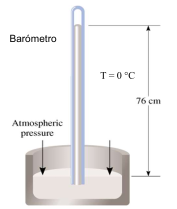
\includegraphics[width=5cm]{./imagenes/barometro.png} \end{center}
            \begin{center} \textcolor{blue}{\underline{Manómetros}} \end{center}
                \sangria{} Son usados para medir la presión de gases distintos a los de la atmósfera.
                \begin{center} 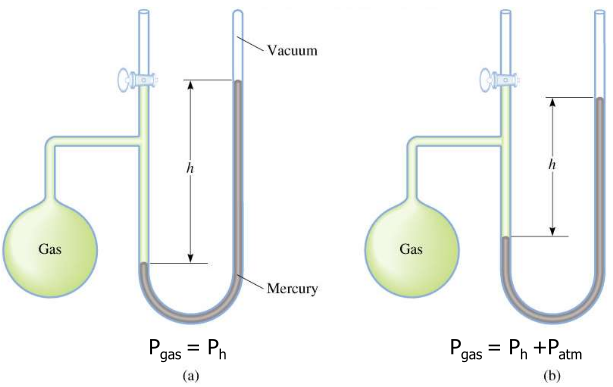
\includegraphics[width=6cm]{./imagenes/manometros.png} \end{center}
        \subsubsection{Leyes de los gases ideales}
            \begin{center} \textcolor{blue}{\underline{Ecuación de los gases ideales}} \end{center} 
            \begin{center}
                $P \cdot V = n \cdot R \cdot T$
            \end{center}
            \sangria{} Siendo:
            \begin{itemize}
                \item $P$ = presión.
                \item $V$ = volumen.
                \item $n$ = moles.
                \item $R$ = constante de los gases ideales.
                \item $T$ = temperatura.
            \end{itemize}
            \begin{center}
                \begin{tabular}{| c |}
                    \hline
                    \textcolor{red}{\textbf{Valores de la const. $R$}} \\
                    \hline
                    0,082057 $atm \cdot L \cdot {mol^{-1}} \cdot {K^{-1}}$ \\
                    \hline
                    8,3145 $m^3 \cdot Pa \cdot {mol^{-1}} \cdot {K^{-1}}$ \\
                    \hline
                    8,3145 $J \cdot {mol^{-1}} \cdot {K^{-1}}$ \\
                    \hline
                \end{tabular}
            \end{center}
            \begin{center} \textcolor{blue}{\underline{Ley de Boyle}} \end{center} 
            \begin{center} 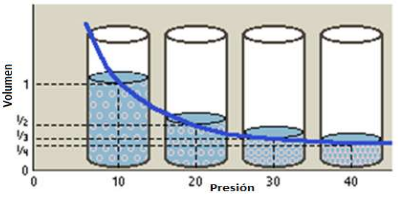
\includegraphics[width=7cm]{./imagenes/graficaLeyBoyle.png} \end{center}
            \sangria{} Para $n$ y $T$ constantes:
            \begin{center} $P \propto \frac{1}{V}$ \end{center}
            \begin{center} $P \cdot V = cte$ \end{center}
            \begin{center} \textcolor{blue}{\underline{Leyes de Charles y Gay-Lussac}} \end{center} 
            \begin{center} 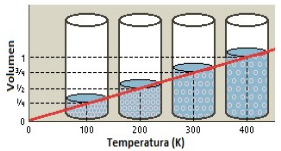
\includegraphics[width=7cm]{./imagenes/graficaLeyCharlesYGayLussac1.png} \end{center}
            \sangria{} Para $n$ y $P$ constantes:
            \begin{center}
                $V \propto T$ \\
                $\frac{V}{T} = cte$
            \end{center}
            \sangria{} Expresión para dos puntos:
            \begin{center} $\frac{V_1}{T_1} = \frac{V_2}{T_2}$ \end{center}
            \sangria{} Para $n$ y $V$ constantes:
            \saltoPag{}
            \begin{center} 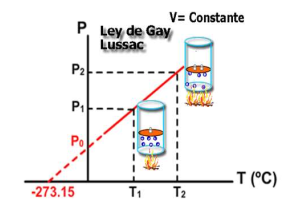
\includegraphics[width=7cm]{./imagenes/graficaLeyCharlesYGayLussac2.png} \end{center}
            \begin{center}
                $P \propto T$ \\
                $\frac{P}{T} = cte$
            \end{center}
            \sangria{} Expresión para dos puntos:
            \begin{center} $\frac{P_1}{T_1} = \frac{P_2}{T_2}$ \end{center}
            \begin{center} \textcolor{blue}{\underline{Ley de Avogadro}} \end{center}
            \begin{center} 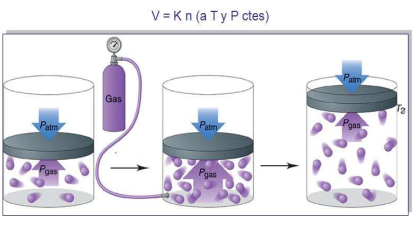
\includegraphics[width=7cm]{./imagenes/dibujoLeyAvogadro.png} \end{center}
            \sangria{} Para $P$ y $T$ constantes:
            \begin{center}
                $V \propto n$ \\
                $\frac{V}{n} = cte$
            \end{center}
            \sangria{} Expresión para dos puntos:
            \begin{center} $\frac{V_1}{n_1} = \frac{V_2}{n_2}$ \end{center}
            \sangria{} En condiciones normales, es decir a $1atm$ y a $\ang{273} K$, $1mol$ de gas = $22,4 L$ de gas.
        \subsubsection{Masa molar y densidad de los gases}
            \sangria{} Para la masa molar, se sabe que:
            \begin{center}
                \begin{tabular}{| c | c |}
                    \hline
                    Ec. Gases ideales & $P \cdot V = n \cdot R \cdot T$ \\
                    \hline
                    Moles & $n = \frac{m}{M}$ \\
                    \hline
                \end{tabular}
            \end{center}
            \sangria{} Donde:
            \begin{itemize}
                \item $n$ = número de moles.
                \item $m$ = masa de la sustancia.
                \item $M$ = masa molar de la sustancia.
            \end{itemize}
            \begin{center}
                $P \cdot V = n \cdot R \cdot T$ \\[5pt]
                $P \cdot V = (\frac{m}{M}) \cdot R \cdot T$ \\[5pt]
                \textcolor{red}{\textbf{$M = \frac{m \cdot R \cdot T}{P \cdot V}$} \hspace{15pt} \textit{\textbf{Masa molar del gas}}}
            \end{center}
            \columnbreak{}
            \sangria{} Para la masa molar, se sabe que:
            \begin{center}
                \begin{tabular}{| c | c |}
                    \hline
                    Ec. Gases ideales & $P \cdot V = n \cdot R \cdot T$ \\
                    \hline
                    Moles & $n = \frac{m}{M}$ \\
                    \hline
                    Densidad & $\delta = \frac{m}{V}$ \\
                    \hline
                \end{tabular}
            \end{center}
            \begin{center}
                $P \cdot V = n \cdot R \cdot T$ \\[5pt]
                $P \cdot V = (\frac{m}{M}) \cdot R \cdot T$ \\[5pt]
                $P \cdot M = \frac{m}{V} \cdot R \cdot T$ \\[5pt]
                $P \cdot M = \delta \cdot R \cdot T$ \\[5pt]
                \textcolor{red}{\textbf{$\delta = \frac{P \cdot M}{R \cdot T}$} \hspace{15pt} \textbf{Densidad de un gas}}
            \end{center}
        \subsubsection{Ley de Dalton para las presiones parciales}
            \begin{center} 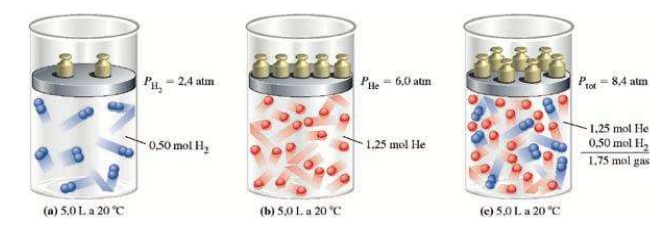
\includegraphics[width=8cm]{./imagenes/dibujoLeyDeDaltonPresionesParciales.png} \end{center}
            \begin{itemize}
                \item Las leyes de los gases se aplican a sustancias puras.
                \item Se define ''Presión parcial'' como: \\
                    \textcolor{red}{Cada componente de una mezcla de gases ejerce una presión igual a la que se ejercería si estuviese él solo en el recipiente.}
            \end{itemize}
            \begin{center}
                $P_{total} = P_1 + P_2 + \dotsb + P_n$
            \end{center}
            \sangria{} Para cada presión parcial, su valor es de:
            \begin{center} $P_1 = n_1 \cdot \frac{R \cdot T}{V}$ \end{center}
            \sangria{} Entonces, la expresión anterior se puede re-escribir como:
            \begin{center}
                $P_{total} = P_1 + P_2 + \dotsb + P_n$ \\[5pt]
                $P_{total} = n_1 \cdot \frac{R \cdot T}{V} + n_2 \cdot \frac{R \cdot T}{V} + \dotsb + n_n \frac{R \cdot T}{V}$ \\[5pt]
                \textcolor{red}{\textbf{$P_{total} = (n_1 + n_2 + \dotsb + n_n) \cdot \frac{R \cdot T}{V}$}}
            \end{center}
            \begin{center} \textcolor{blue}{\underline{Fracciones molares ($X$)}} \end{center}
            \sangria{} Siendo:
            \begin{center}
                $P_1 = n_1 \cdot \frac{R \cdot T}{V}$ \\[5pt]
                $P_T = n_T \cdot \frac{R \cdot T}{V}$ \\[5pt]
                $\frac{P_1}{P_T} = \frac{n_1}{n_T} = X_1$ \\[5pt]
                \textcolor{red}{\textbf{$P_1 = X_1 \cdot P_T$}} \\[5pt]
                \textcolor{red}{\textbf{$X_1 + X_2 + \dotsb + X_n = 1$}}
            \end{center}
        \subsubsection{Teoría cinética molecular}
            \sangria{} Los gases están formados por un gran número de moléculas que se mueven de modo continuo y aleatorio.
            \saltoPag{}
            \begin{itemize}
                \item Las moléculas están separadas por distancias mayores a sus dimensiones, se las considera como puntos (tienen masa y su volumen es insignificante).
                \item Las moléculas chocan con las pareces del recipiente y entre sí. Los choques entre moléculas es en forma elástica, toda energía se transfiere de una molécula a otra. La energía total de las moléculas no cambia.
                \item Las moléculas no ejercen entre sí fuerzas de atracción o repulsión.
                \item La energía cinética promedio de las moléculas es proporcional a la temperatura absoluta. A cualquier temperatura dada, dos gases tienen igual energía cinética promedio:
                \begin{center} $KE = \frac{1}{2} m u^2$ \end{center}
                \sangria{} La presión de un gas es resultado de las colisiones entre las moléculas y las paredes del recipiente. Depende de la frecuencia de las colisiones por unidad de área y de la fuerza de las moléculas al chocar las paredes. La temperatura absoluta es una medida de la energía cinética promedio de las moléculas, es decir, del movimiento aleatorio.
            \end{itemize}
            \begin{center} \textcolor{red}{\underline{Aplicación de las leyes de los gases}} \end{center}
            \begin{center} 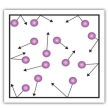
\includegraphics[width=4cm]{./imagenes/colisionesParticulas.png} \end{center}
            \begin{itemize}
                \item Compresibilidad de los gases.
                \item Ley de Boyle: \\[2pt]
                    \sangria{} La $P$ es $\propto$ al número de colisiones con las paredes del recipiente. El número de colisiones es $\propto$ a la densidad del gas; al disminuir el $V$ aumenta la densidad ($\frac{1}{V}$), por lo tanto la presión $P$ es $\propto \frac{1}{V}$.
                \item Ley de Charles: \\[2pt]
                    \sangria{} La energía cinética promedio es $\propto T$:\\[2pt]
                    \sangria{} Al aumentar la $T$, aumenta el número y la fuerza de las colisiones generando más presión ($P \propto T$). Si el volumen del gas se expande, la presión se equilibra con la externa por lo que $V \propto T$.
                \item Hipótesis de Avogadro:\\[2pt]
                    \sangria{} Se demostró que la $P$ es $\propto$ a la densidad y a la $T$. Como la masa del gas es $\propto$ al número de moles ($n$) del gas, la densidad se expresa como $\frac{n}{V}$. Por lo tanto:
                    \columnbreak{}
                    \begin{center} 
                        $P \propto (\frac{n}{V} \cdot T = C (\frac{n}{V}) T)$
                    \end{center}
                    Donde $C$ es una constante de proporcionalidad. Dos gases a la misma $T$, $P$ y $V$ tendrán la misma cantidad de moles.
                \item Ley de Dalton de las presiones parciales:\\[2pt]
                    \sangria{} Las moléculas no se atraen ni se repelen. La presión creada por un tipo de molécula no es afectada por la presencia de otro gas. 
                    \begin{center} $P_{total} = \sum P_i$ \end{center}
            \end{itemize}
        \subsubsection{Difusión y efusión}
            \begin{center}
                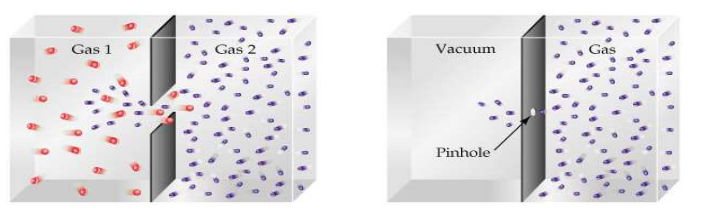
\includegraphics[width=6cm]{./imagenes/difusionEfusion1.png} \\
                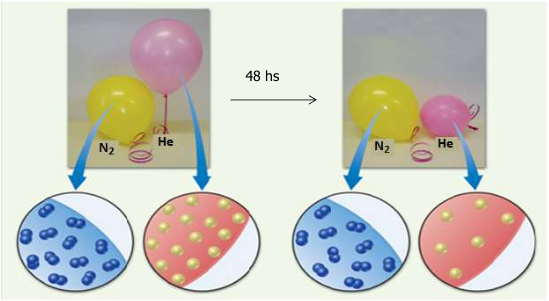
\includegraphics[width=7cm]{./imagenes/difusionEfusion2.png}
            \end{center}
            \begin{center} \textcolor{red}{\underline{Ley de Graham}} \end{center}
            \begin{center}  $\frac{r_1}{r_2} = \sqrt{\frac{M_2}{M_1}}$ \end{center}
            \sangria{} Siendo:
            \begin{itemize}
                \item $r_1$ y $r_2$: velocidades de difusión o efusión de los gases.
                \item $M_1$ y $M_2$: masas molares de los gases correspondientes.
            \end{itemize}
            \underline{\textbf{Ejercicio:}} Le toma 192 segundos a un gas desconocido para efundirse a través de una pared porosa y 84 segundos al mismo volumen de Nitrógeno efundirse a la misma temperatura y presión ¿Cuál es la masa molar del gas desconocido?
            \begin{center} 
                $\frac{r_1}{r_2} = \frac{\sqrt{M_2}}{\sqrt{M_1}}$ \\[5pt]
            \end{center}
            Se sabe que:
            \begin{center} $r_1 = \frac{1}{t_1}$ \end{center}
            \begin{center} $t_1 = \frac{1}{r_1}$ \end{center}
            \begin{center} $\frac{t_2}{t_1} = \frac{\sqrt{M_2}}{\sqrt{M_1}}$ \end{center}
            \begin{center} $M_2 = \frac{t_2}{t_1} \cdot \sqrt{M_1}$ \end{center}
            \begin{center} $M_2 = \frac{142s}{84s} \cdot \sqrt{28 g/mol}$ \end{center}
            \begin{center} \begin{tabular}{| c |} \hline $M_2 = 146,3 g/mol$ \\ \hline \end{tabular} \end{center}
        \saltoPag{}
        \subsubsection{Gases reales: desviaciones del comportamiento real}
            \sangria{} Un gas se acerca a un comportamiento ''ideal'' cuando su factor de compresibilidad es $1$ o cercano a este:
            \begin{center} $\frac{P \cdot V}{R \cdot T} = 1$ \end{center}
            \begin{center} 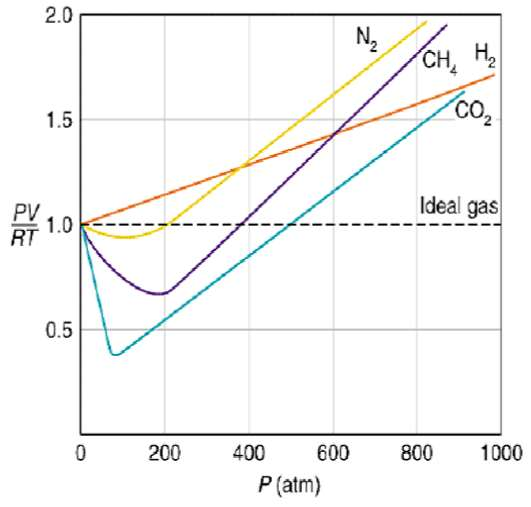
\includegraphics[width=6cm]{./imagenes/factorDeCompresibilidadVSPresion.png} \\ \textit{A presiones bajas se puede usar la ecuación del gas ideal sin generar errores graves.} \end{center}
            \sangria{} A temperaturas elevadas, los gases reales se comportan como ideales:
            \begin{center} 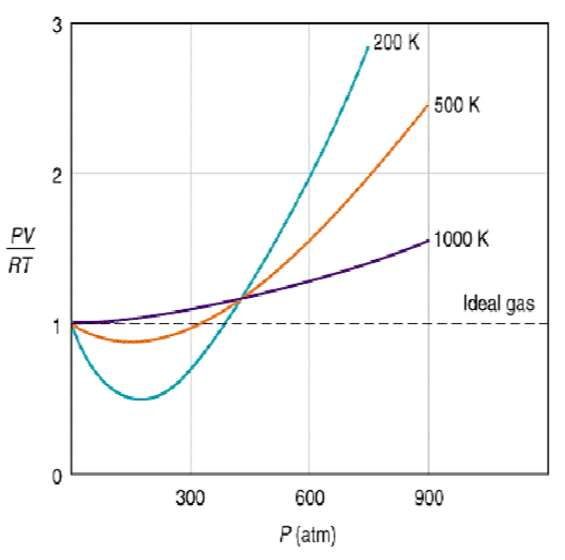
\includegraphics[width=6cm]{./imagenes/gasIdealATemperatuasAltas.png} \\ \textit{Curvas de 1 mol de $N_2$} \end{center}
            \sangria{} A presiones altas, el volumen del gas no es despreciable frente al del recipiente. Las fuerzas de atracción son apreciables.
            \begin{center} 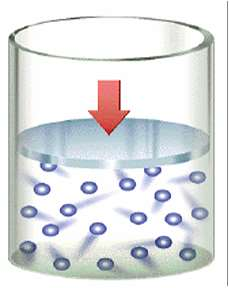
\includegraphics[width=2cm]{./imagenes/presionesAltasGasIdeal1.png}\hspace{1cm}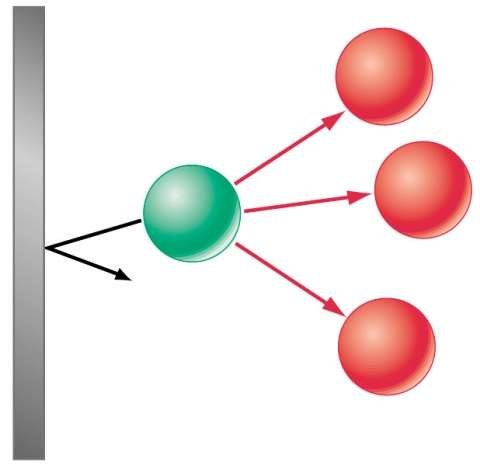
\includegraphics[width=2cm]{./imagenes/presionesAltasGasIdeal2.png} \end{center}
            \begin{center} \textbf{\underline{Ecuación de Van der Waals}} \end{center}
            \begin{center} $P_{ideal} = P + \frac{a \cdot n^2}{V^2}$ \end{center}
            \begin{center} \begin{tabular}{| c |} \hline $(P_real + \frac{a \cdot n^2}{V^2}) (V -n \cdot b) = n \cdot R \cdot T$ \\ \hline \end{tabular} \end{center}
            \columnbreak{}
            \sangria{} Siendo:
            \begin{itemize}
                \item $P_{real}$: presión del gas real.
                \item $V$: volumen del gas.
                \item $n$: número de moles del gas.
                \item $R$: constante de los gases ideales.
                \item $T$: temperatura en Kelvin.
                \item $a$: corrección por las fuerzas inter-moleculares. Aumente para gases con interacciones más fuertes.
                \item $b$: corrección por el volumen finito de las moléculas; reduce el volumen disponible.
            \end{itemize}
            \begin{center} \textcolor{red}{\underline{Constantes de Van der Waals}}\\[5pt] 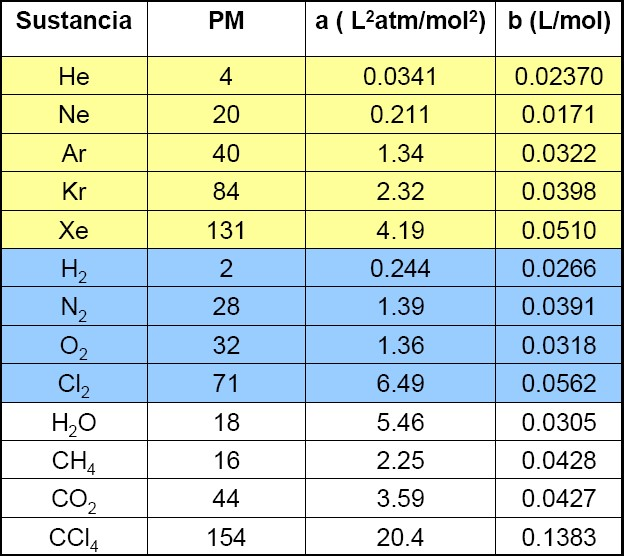
\includegraphics[width=6cm]{./imagenes/constantesVannDerWaals.png} \end{center}
    \subsection{Sólidos}
        \subsubsection{Características de los sólidos}
            \begin{itemize}
                \item Las partículas que lo forman se encuentran ordenadas espacialmente, ocupando posiciones fijas, dando lugar a una estructura interna cristalina, debido a que las fuerzas inter-moleculares son muy fuertes.
                \item Las fuerzas responsables de la estabilidad de un cristal pueden ser iónicas, covalentes, de Van der Waals, de enlaces de hidrógeno o una combinación de todas ellas.
                \item Las partículas pueden ser: moléculas, átomos o iones.
            \end{itemize}
        \subsubsection{Redes y celda unidad}
            \begin{itemize}
                \item \textbf{Red cristalina:} es un ordenamiento infinito de puntos en el espacio, en el que cada punto tiene idéntico entorno.
                \item \textbf{Estructura cristalina:} es el ordenamiento periódico de átomos en un cristal.
                \item Cada cristal deriva de un bloque de construcción básico (''ladrillo'') que se repite en todas las direcciones del espacio. Este bloque de construcción se denomina \textbf{Celda unidad}.
                \item Una celda unitaria es la unidad estructural repetida de un sólido cristalino.
            \end{itemize}
            \saltoPag{}
            \begin{center} 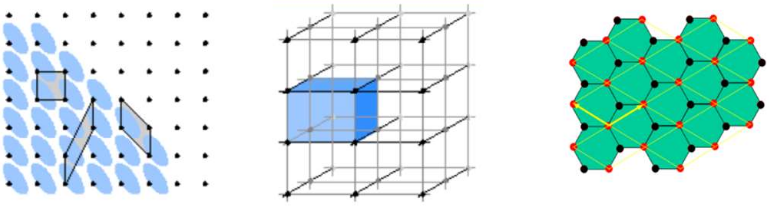
\includegraphics[width=7cm]{./imagenes/celdaUnitaria.png} \end{center}
            \begin{center} 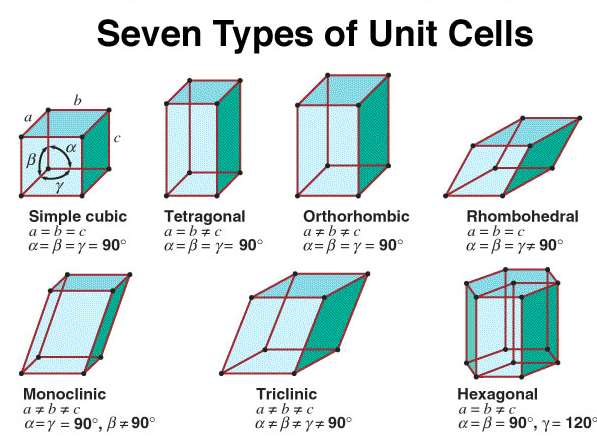
\includegraphics[width=7cm]{./imagenes/tiposDeCeldas.png} \end{center}
            \begin{center} 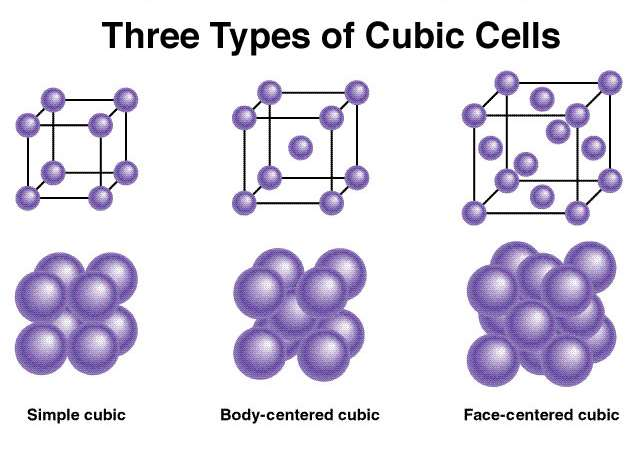
\includegraphics[width=7cm]{./imagenes/tiposDeCeldasCubicas.png} \end{center}
            \begin{center} 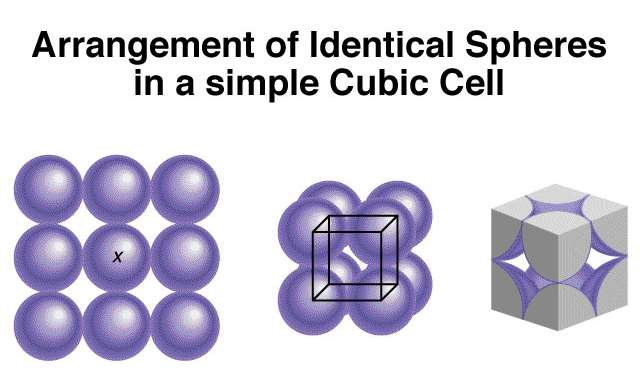
\includegraphics[width=7cm]{./imagenes/celdaCubicaSimple.png} \end{center}
            \begin{center} 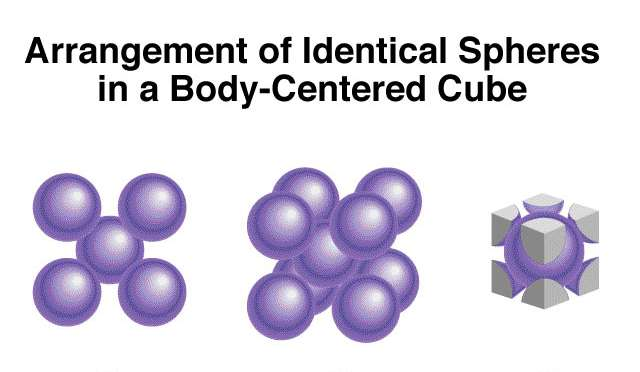
\includegraphics[width=7cm]{./imagenes/celdaCubicaCentradaEnElCuerpo.png} \end{center}
            \begin{center} 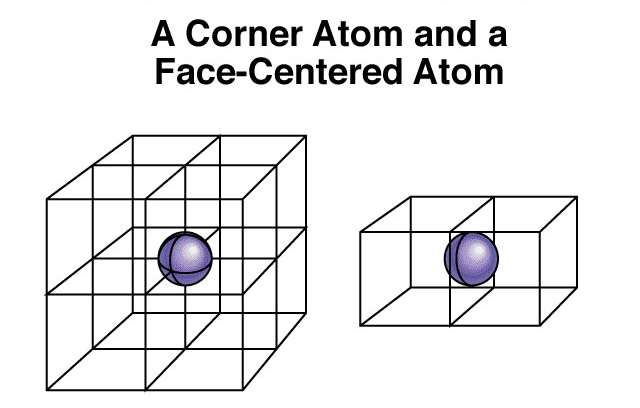
\includegraphics[width=7cm]{./imagenes/distribucionAtomosVerticeYCaraCeldaUnitaria.png} \end{center}
            \begin{center} 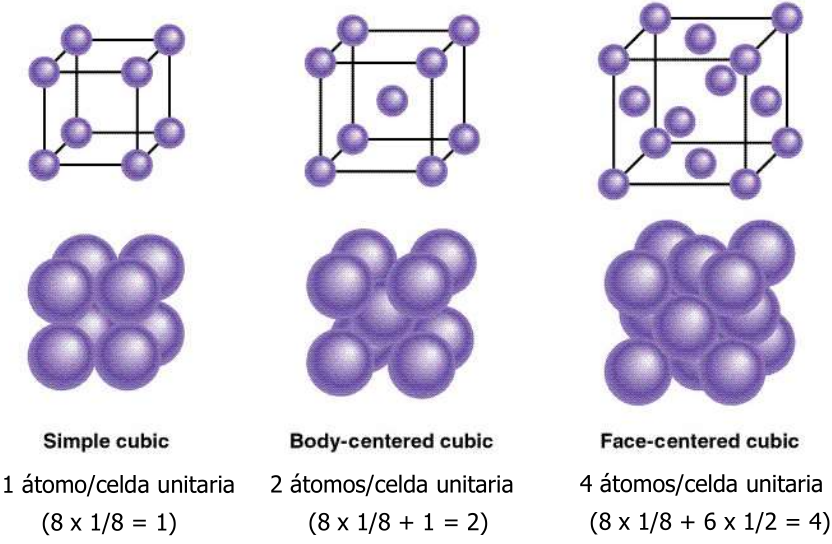
\includegraphics[width=7cm]{./imagenes/atomosEnCeldasUnitarias.png} \end{center}
            \begin{center} \textcolor{red}{\underline{Empaquetamiento compacto}} \end{center}
            \begin{center} 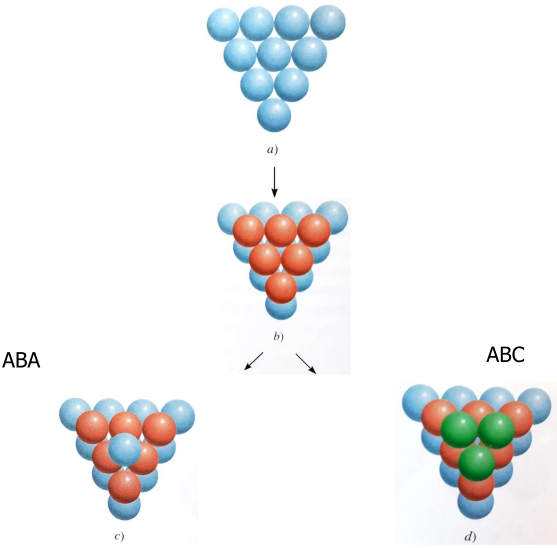
\includegraphics[width=7cm]{./imagenes/empaquetamientoCompacto.png} \end{center}
            \begin{center} \textcolor{red}{\underline{Empaquetamiento de esferas}} \end{center}
            \begin{center} 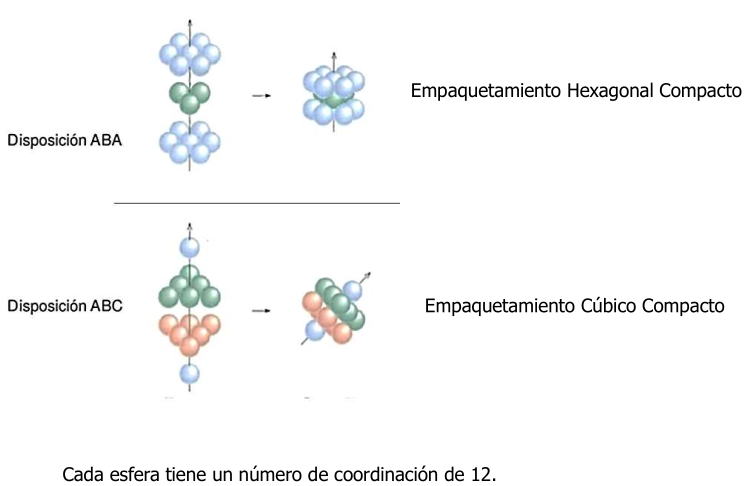
\includegraphics[width=7cm]{./imagenes/empaquetamientoDeEsferas.png} \end{center}
            \sangria{} Conceptos:
            \begin{itemize}
                \item \textbf{Número de coordinación:} número de vecinos o átomos más cercanos.
                \item \textbf{Factor de empaquetamiento:} es la fracción del espacio ocupara por los átomos en la celda.
                \item \textbf{Direcciones compactas:} sentido dentro de un cristal a lo largo de los cuales los átomos están en contacto.
            \end{itemize}
            \saltoPag{}
            \textbf{Contenido de la celda unidad}
            \begin{center} 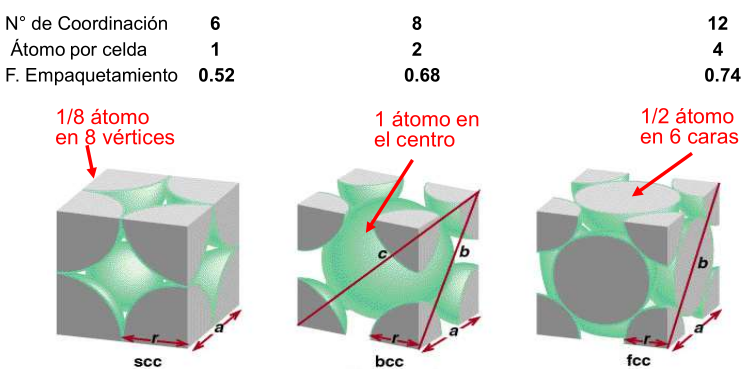
\includegraphics[width=7cm]{./imagenes/contenidoCeldaUnidad.png} \end{center}
            \begin{center} \textcolor{red}{\underline{Densidad de un sólido cristalino}} \end{center}
            \begin{center} $\rho = \frac{n \cdot M}{V_C \cdot N_A}$ \end{center}
            Siendo:
            \begin{itemize}
                \item $n$: $n^o$ átomos/celda unidad.
                \item $M$: peso atómico ($g/mol$).
                \item $V_C$: volumen celda unidad ($cm^3$).
                \item $N_A$: número de Avogadro ($6,023 \times 10^{23}$)
            \end{itemize}
            \sangria{} Por ejemplo, cuando la plata se cristaliza, forma celdas cúbicas de cara centrada. La longitud de la arista de la celda unitaria es de $409pm$. Si quisiéramos calcular la densidad de la plata:
            \begin{center} $d = \frac{m}{v}$ \\[5pt] $V = a^3 = (409pm)^3 = 6,83 \times 10^{-23} cm^3$ \end{center}
            $4$ átomos/celda unitaria en una celda cúbica de cara centrada.
            \begin{center}
                $m = 4 \text{Ag átomos} \times \frac{107,9g}{molAg} \times \frac{1molAg}{6,022 \times 10^{23} \text{átomos}}$ \\[5pt] $ m = 7,17 \times 10^{-22}g$ \\[10pt] $d = \frac{m}{v}$ \\[5pt] $d = \frac{7,17 \times 10^{-22}g}{6,83 \times 10^{-23}cm^3}$ \\[5pt]
                \begin{tabular}{| c |} \hline $d = 10,5 g/cm^3$ \\ \hline \end{tabular}
            \end{center}
        \subsubsection{Tipos de sólidos}
            \begin{itemize}
                \item \textbf{Sólidos metálicos:} \\
                    \sangria{} Los metales son sistemas sólidos integrados por átomos unidos por fuerzas de enlace metálico. Cada punto reticular del cristal está formado por un átomo del mismo metal. En general, presentan alta conductividad eléctrica y térmica.
                    \begin{center} 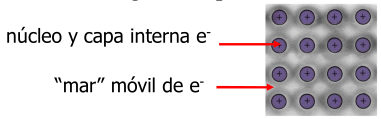
\includegraphics[width=3cm]{./imagenes/solidosMetalicos.png} \end{center}
                \item \textbf{Sólidos covalentes:} \\
                    \sangria{} Son sólidos con un ordenamiento tridimensional en el que existen enlaces covalentes entre todas las unidades estructurales. Son los sólidos de mayor dureza. Tienen alto punto de fusión. Ejemplos: diamantes, grafito, $SiO_2$, $SiC$.
            \end{itemize}
        \subsubsection{Tipos de cristales}
            \begin{center} 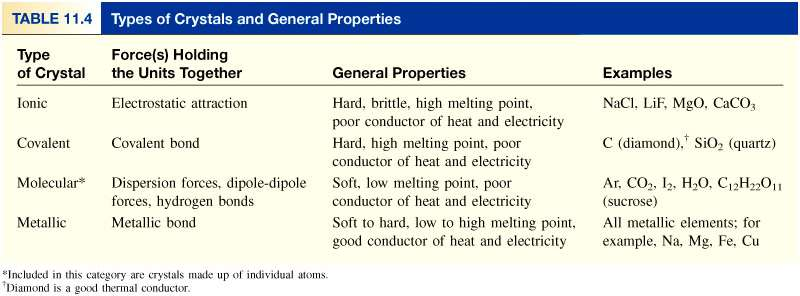
\includegraphics[width=8cm]{./imagenes/tiposDeCristales.png} \end{center}
        \subsubsection{Teoría de bandas de conducción}
            \sangria{} En la teoría de la conductividad de las bandas, los electrones des-localizados se mueven libremente a través de ''bandas'' formadas por orbitales moleculares tralapados.
            \begin{center} 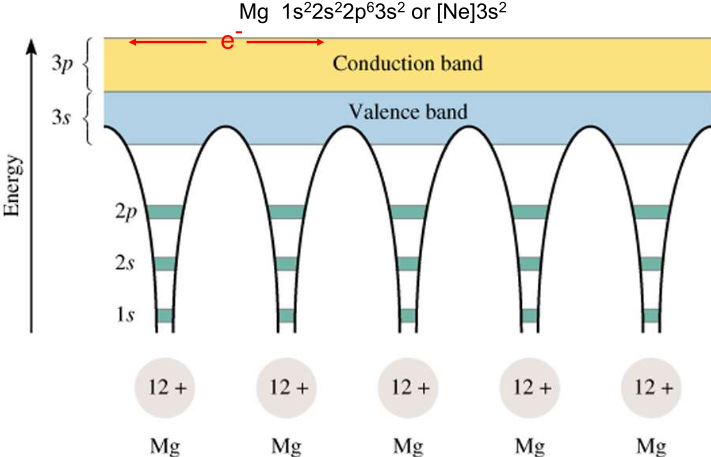
\includegraphics[width=8cm]{./imagenes/bandasDeConduccionMg.png} \end{center}
        \begin{center} \textcolor{red}{\underline{Espacios de energía entre valencia y bandas} \underline{conductivas en metales, semi-conductores y aislantes}} \end{center}
        \begin{center} 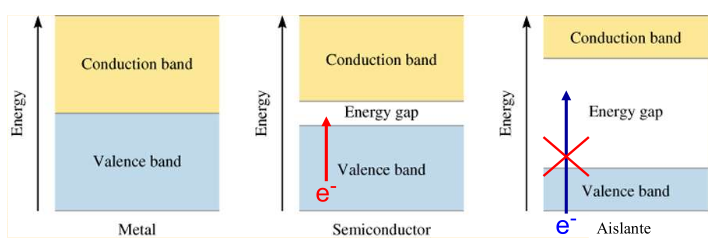
\includegraphics[width=8cm]{./imagenes/espaciosEnergiaValenciaYBandasConductivasMetales.png} \end{center}
        \begin{itemize}
            \item \textbf{Semiconductor intrínseco:} elemento semiconductor puro.
            \item \textbf{Semiconductor extrínseco:} cuando el semiconductor está dopado con átomos de otro elemento disminuyendo la brecha energética prohibida.
        \end{itemize}
        \begin{center} \textcolor{red}{\underline{Semiconductores (tipos)}} \end{center}
        \begin{center} 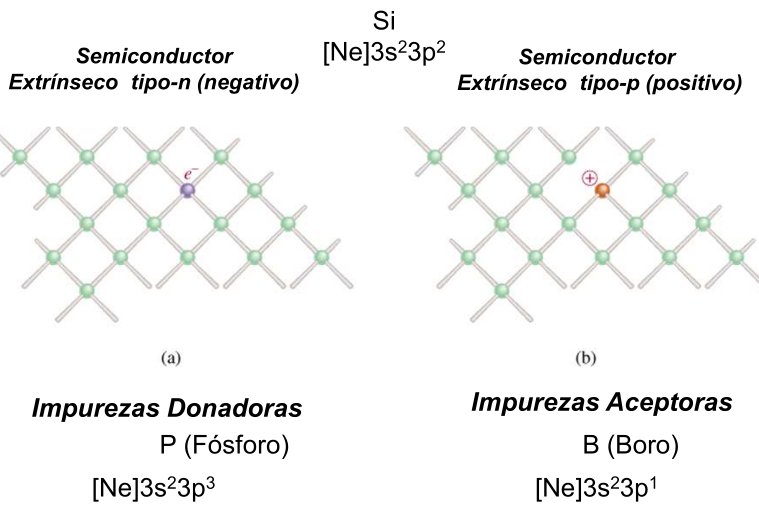
\includegraphics[width=8cm]{./imagenes/tiposSemiconductores.png} \end{center}
        \saltoPag{}
        \begin{center} 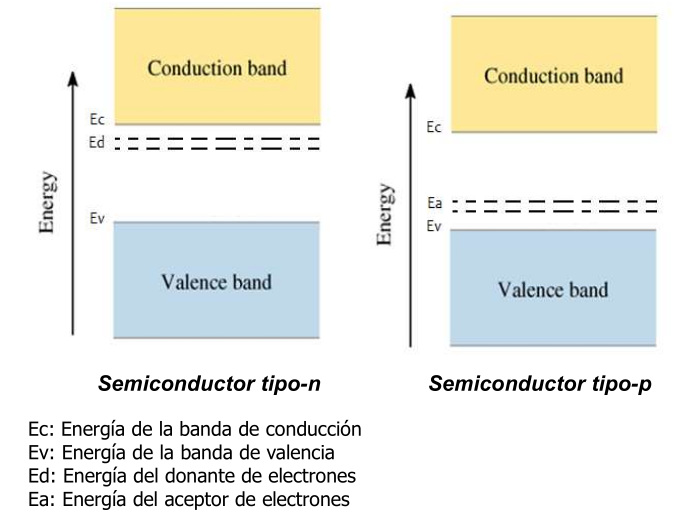
\includegraphics[width=8cm]{./imagenes/tiposSemiconductores1.png} \end{center}
        


    

